\documentclass{article}
\usepackage{amsmath,amssymb}
\usepackage{hyperref}
\usepackage{graphicx}
\usepackage{todonotes}

\title{\bf{Laboratory Project Two: Calibration of an Oriface Meter}}
\author{Jon Langston \& Nicholas Malaya \& Owen O'Neal \\ Department of Mechanical Engineering \\ University of Texas at Austin} \date{}

\begin{document}
\maketitle
\date{}
\newpage
\section{Presentation of Calibration Data}

\textbf{A calibration of the $C_d$ vs $Re$ and comment on whether your
results were as expected.}   

We have adjusted the sample rates down  300 samples at a rate of 100
Hz. The results are shown in Figure 
\ref{oriface-time}, below. The samples appear to still be correlated in
time. 

\begin{figure}[!htb]
  \begin{center}
    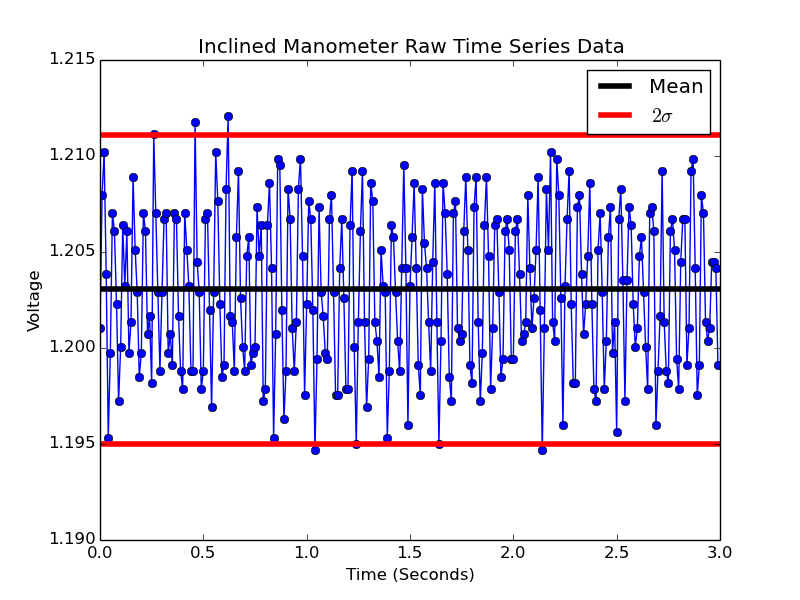
\includegraphics[width = 12 cm]{figs/oriface_time.png}
    \caption{Example raw time series data from a single oriface meter 
      run. The calculated mean of the signal is shown in black, along with
      the two $\sigma$ (standard deviation) confidence interval in
      red.}
    \label{oriface-time}
  \end{center}
\end{figure}

Let's go deeper, and look at the samples over a shorter period of time. Instead of the full 3 
second sampling time, we examine just 0.4 seconds. The result of this is shown in \ref{oriface-time-4}.
From this perspective, it appears we are still indeed oversampling, as at least subsequent points 
tend to be correlated with each other. 

\begin{figure}[!htb]
  \begin{center}
    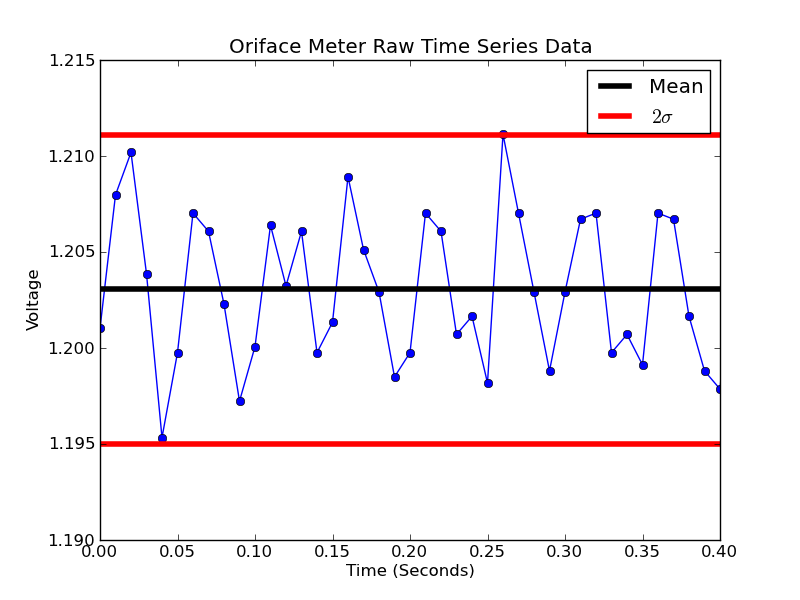
\includegraphics[width = 12 cm]{figs/oriface_time_04.png}
    \caption{Example raw time series data from a single oriface meter 
      run, plotted over a shorter time period.}
    \label{oriface-time-4}
  \end{center}
\end{figure}


Examining the probability distribution functions in Figure \ref{oriface-hist},
we can see that while the results are clearly better than the other lab, where we used 1000 Hz and 1000 samples. 
However, while these results are closer to that of a gaussian, 
they are still not normally distributed. In other words, we still have not found an ideal data sampling rate 
for the pressure transducer.  

  \begin{figure}[!htb]
   \begin{center}
    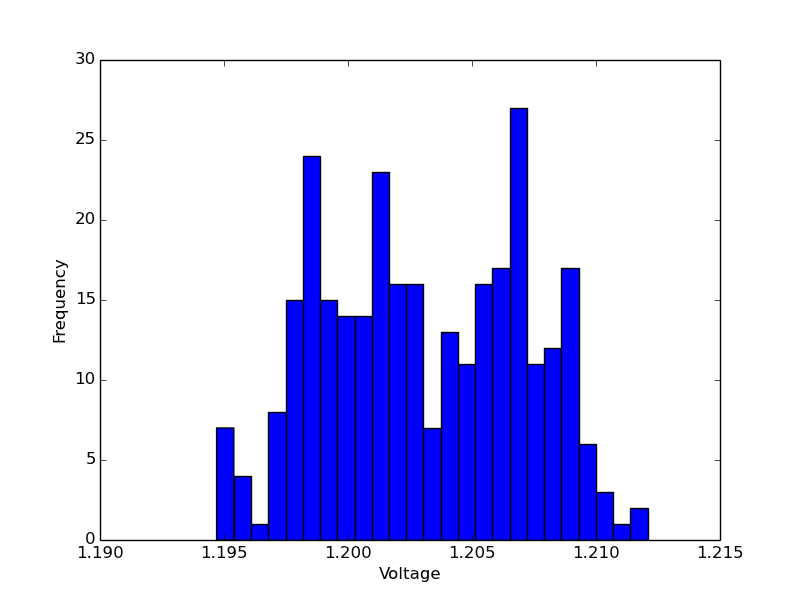
\includegraphics[width = 12 cm]{figs/oriface_hist.png}
    \caption{Histogram depicting the frequency of voltages in our
    signal. This was generated with fifty bins, but the results did not
    appear to be sensitive to the number selected.}
    \label{oriface-hist}
   \end{center}
  \end{figure}

We proceed with our calculations of the quantities of interest. We
intend to plot $C_d$ as a function of Reynolds number. We have not made
a direct measurement of either quantity, and must calculate them as
surrogate quantities from our data. 

The Reynolds number is defined as, 
\begin{equation}
 \text{Re} = \frac{UL}{\nu}.
\end{equation}

The kinematic viscosity ($\nu$) and the oriface diameter ($L$) are
given. We can calculate the bulk fluid velocity ($U$) from our knowledge
of the flow rate and the system dimensions, 
\begin{equation}
 U = \frac{Q}{A} = \frac{Q}{\pi r^2} = \frac{Q}{\pi d^2/4}.
\end{equation}
The Reynolds number is therefore calculated as,
\begin{equation}
 Re = \frac{Q L}{\pi \nu d^2/4}.
\end{equation}

Turning our attention to the calibration coefficient, Equation (9.2)
from page 211 in Stavros' text describes a relation for  
the flow rate as a function of the pressure drop,  
\begin{equation*}
 Q = C_d \frac{\pi d^2 / 4}{\sqrt{1-(d/D)^4}}\sqrt{\frac{2 \Delta p}{\rho}}.
\end{equation*}
This can be manipulated to provide an equation for $C_d$ as, 
\begin{equation}
 C_d = \frac{Q (1-\beta^4)^{1/2}}{\pi d^2/4} \left(\frac{\rho}{2 \Delta
					      P}\right)^{1/2}.
\end{equation}

The results of $C_d$ vs. Re are plotted in Figure \ref{orif}. We can see a general trend of increasing 
values of $C_d$ as a function of $Re$, followed by the curve ``flattening out''. For flow in a duct, 
the transition between laminar and turbulent flow occurs around a few thousand Re, so the vast majority 
of our data lies in the turbulent regime. Our expectation is that the $C_d$ becomes independent of Re at high 
(e.g. turbulent) Re, and the data appears to be consistent with this. The value of $C_d$ asymptotes to a value near 0.6, which is roughly in line with values we found in the literature for these aspect ratios ($\beta$ values).

  \begin{figure}[!htb]
   \begin{center}
    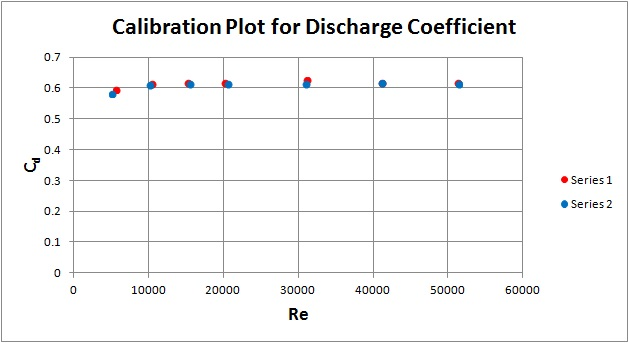
\includegraphics[width = 12 cm]{figs/cd_v_re_zero_axis.jpg}
    \caption{A plot of $C_d$ as a function of Reynolds Number. Only the first point is likely to be 
outside of the fully developed turbulence regime. }
    \label{orif}
   \end{center}
  \end{figure}

  \begin{figure}[!htb]
   \begin{center}
    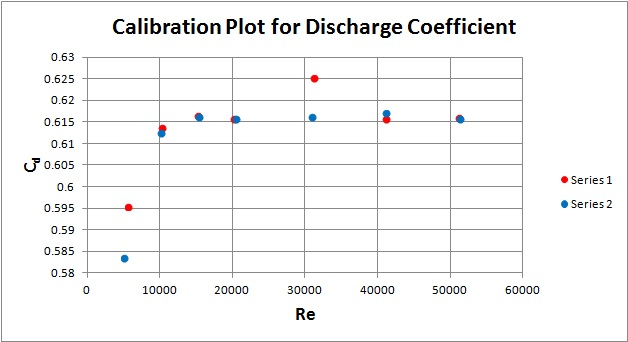
\includegraphics[width = 12 cm]{figs/cd_v_re.jpg}
    \caption{A plot of $C_d$ as a function of Reynolds Number. This plot is zoomed into the region of the data, 
    to make the difference between points more pronounced.}
    \label{orif-zoom}
   \end{center}
  \end{figure}

The first data point, as previously mentioned, appears to be anomalously low. The value of this point is 
still high enough ($\approx 5000$) that we would expect it to be turbulent. However, it is possibly close enough 
to the transition that it is not yet fully developed. A zoomed in version of this plot is shown in figure \ref{orif-zoom}. 

\newpage
\section{Uncertainty Analysis}

\textbf{Uncertainty of flow rate measured using the orifice meter with
your calibration.} 

Taking the differences in pressure measured across the laminar flow element and orifice meter, 
we can calculate the discharge coefficient using the equations below. The average discharge coefficient 
calculated from our pressure measurements was nominally 0.615 across both series.

\begin{equation}
  C_d = \frac{Q_{\text{LFE}} }{A_0} * (1-\beta^4)^{1/2} * \left(\frac{\rho}{\Delta P_{\text{trans}}}\right)^{1/2}
\end{equation}
where, 
\begin{equation}
  Q_{\text{LFE}} = 20.5 \Delta P_{\text{LFE}} * \frac{\mu(21 C)}{\mu(\text{actual})}
\end{equation}

The uncertainty in the discharge coefficient, $U_{C_d}$, has contributions from the uncertainties in
the flow rate, $U_Q$, measured from the laminar flow element and the change in pressure, $U_{\Delta P}$, 
measured from the pressure transducer. We can neglect uncertainties in the area of the orifice, $A_o$, 
and the ratio of diameters from the pipe and orifice meter, $\beta$, because they are taken into account 
when calibrating $C_d$ as a correction factor. Changes in the density of air, $\rho$, are neglected because our 
reynolds number while turbulent should remain well below Mach 0.3.

Neglecting uncertainties in $A_o$, $\beta$, and $\rho$, the percent error for $C_d$ can be expressed as:
\begin{equation}
  \frac{U_{C_d}}{C_d} = \sqrt{ \left(\frac{U_{Q}}{Q}\right)^2 + \left( 0.5 \frac{U_{C_d}}{C_d} \right)^2}
\end{equation}

For the subsequent calculations, we assume $U_Q$ and $U_{\Delta P}$ are bias uncertainties and cannot be 
made more accurate by taking multiple measurements. Taking the specifications given in the lab 
guidelines, $U_{\Delta P}$ is assumed to be a constant 0.002 in. H20. $U_Q$ is a piecewise function equal to 
0.2\%*RDG from $10-100\%$ FS and 0.02\%*FS below 10\% FS. Full scale for the laminar flow element is 160 
CFM, so the measurements at 5, 10, and 15 CFM use this latter value for uncertainty.

Results: 
\begin{itemize}
\item Series 1: $\frac{U_{C_d}}{C_d} = 0.066$ @ 5 CFM and 0.0021 @ 50 CFM
\item Series 2: $\frac{U_{C_d}}{C_d} = 0.076$ @ 5 CFM and 0.0021 @ 50 CFM
\end{itemize}

  \begin{figure}[!htb]
   \begin{center}
    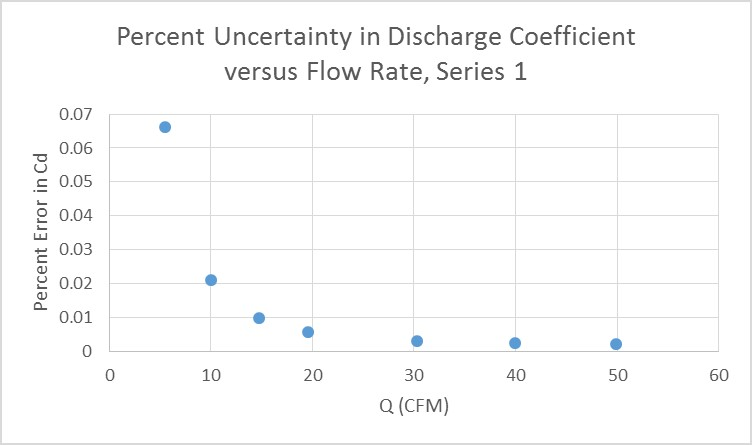
\includegraphics[width = 12 cm]{figs/PercentUncertaintyCdVsQ_Series1.jpg}
    \caption{The uncertainty quantification for discharge coefficient, $C_d$ for the first series of measurements.}
    \label{orif-s1}
   \end{center}
  \end{figure}

  \begin{figure}[!htb]
   \begin{center}
    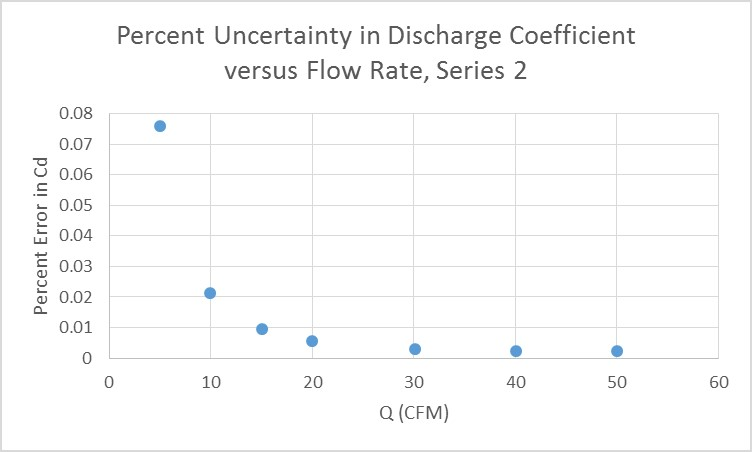
\includegraphics[width = 12 cm]{figs/PercentUncertaintyCdVsQ_Series2.jpg}
    \caption{The uncertainty quantification for discharge coefficient, $C_d$ for the second series of measurements.}
    \label{orif-s2}
   \end{center}
  \end{figure}

Both series of measurements showed the percent error of Cd decreasing exponentially as flow 
rate increased. Upon examination of our sources of error this makes sense. At low flow rates, i.e. Q < 15 
CFM, we need to detect a smaller change in pressure. The constant uncertainty of 0.002 in H20 for our 
pressure transducer is a much greater percentage of the pressure readings at these low flow rates. The 
change in pressure increases non-linearly as flow rate increases, and so at high CFMs the percent error is 
not as significant.

Having calibrated the orifice meter by determining the best obtainable value for $C_d$, we can 
calculate the uncertainty of subsequent measurements of flow rate, $Q_{\text{orifice}}$, using this device.

\begin{equation}
  Q_{\text{orifice}} = \frac{C_d * A_0}{(1-\beta^4)^{1/2}} \left(\frac{2 \Delta P_{\text{trans}}}{\rho}\right)^{1/2}
\end{equation}

Neglecting uncertainties in $A_o$, $\beta$, and $\rho$, the percent error for $Q_{\text{orifice}}$ 
can be expressed using the equation below. Uncertainties for Q were calculated 
assuming a best and worst case scenario: where $U_{\Delta P}$ is a precision
 and bias uncertainty, respectively.

\begin{equation}
  \frac{U_{Q}}{Q} = \sqrt{ \left(\frac{U_{C_d}}{C_d}\right)^2 + \left( 0.5 \frac{U_{\Delta P}}{\Delta P} \right)^2}
\end{equation}

Results:
\begin{itemize}
\item Series 1: Worst: $\frac{U_Q}{Q} = 0.093$ @ 5CFM and 0.0023 @ 50 CFM
\item Series 1: Best:  $\frac{U_Q}{Q} = 0.066$ @ 5CFM and 0.00084 @ 50 CFM
\item Series 2: Worst: $\frac{U_Q}{Q} = 0.11$ @ 5CFM and 0.0023 @ 50 CFM
\item Series 2: Best:  $\frac{U_Q}{Q} = 0.076$ @ 5CFM and 0.00084 @ 50 CFM
\end{itemize}

These results show a similar trend as the uncertainty of the discharge coefficient, decreasing 
exponentially as flow rate increases. For flow rates above 20 CFM, both series predict an uncertainty 
well below 1\% of the flow rate measurement from the orifice meter.

  \begin{figure}[!htb]
   \begin{center}
    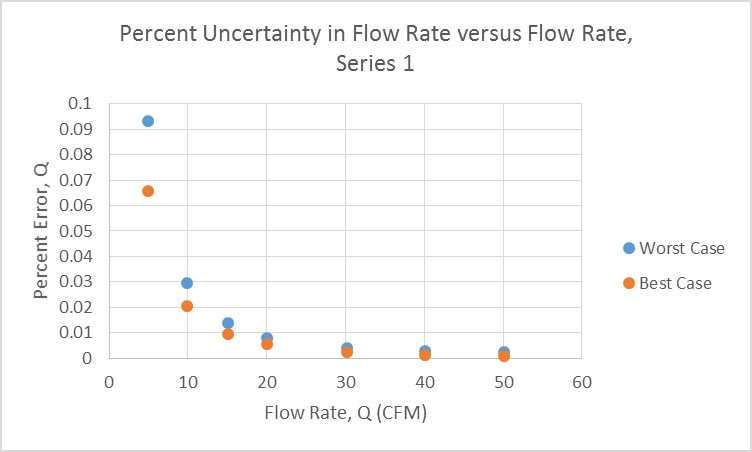
\includegraphics[width = 12 cm]{figs/PercentUncertaintyQVsQ_Series1.jpg}
    \caption{The uncertainty quantification for flow rate, $Q$ for the first series of measurements.}
    \label{orif-s1}
   \end{center}
  \end{figure}

  \begin{figure}[!htb]
   \begin{center}
    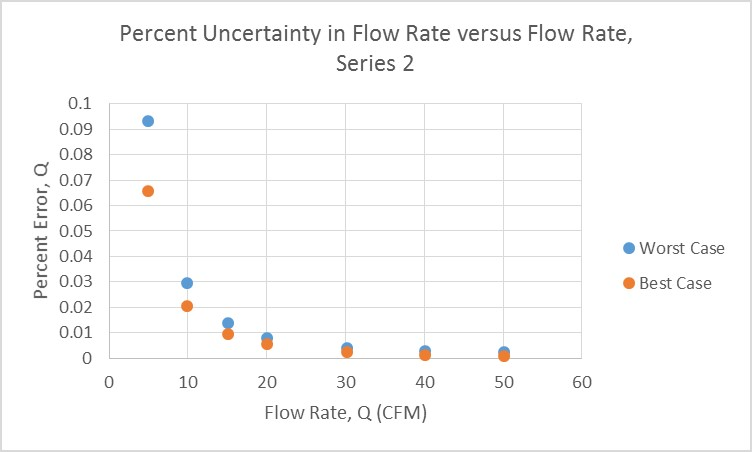
\includegraphics[width = 12 cm]{figs/PercentUncertaintyQVsQ_Series2.jpg}
    \caption{The uncertainty quantification for flow rate, $Q$ for the second series of measurements.}
    \label{orif-s2}
   \end{center}
  \end{figure}

%
%
%
\end{document}

% LocalWords:  reynolds H20 piecewise RDG
